\chapter{\color{Millum}\textbf{Design og utforming}}
I dette kapittelet gjør vi rede for vår prosess tilknyttet utforming og noen av de konkrete designvalgene vi har gjort for å hjelpe brukeren i løsningen.

\section{\textbf{Fremgangsmåte}}
Ved å bruke en fremgangsmåte kalt \textit{Minimum Viable Product} har vi hatt muligheten til å lage et grunnskall for applikasjonen hvor mye av kjernefunksjonaliteten er på plass før vi definerer uttrykket. Ved å bruke denne fremgangsmåten har vi hatt mer tid til å konseptualisere og skissere uttrykkene i applikasjonen

\section{\textbf{Farger}}
Siden mobilapplikasjonen er en utvidelse av Millum Procurement og oppdragsgivers produktportefølje har vi valgt å følge deler av deres fargepalett (\textbf{\ref{fig:farger}}) samt operativsystemene sine egne farger for søkefelter og lignende. Primærfargen kalles for \textbf{Millum Blue} og er en kraftig blåfarge som skal brukes der man ønsker brukerens oppmerksomhet, for eksempel viktige knapper som ``tell`` eller ``lagre``. Sekundærfargen kalles \textbf{Extra Dark Gray}, som er en mørk gråfarge skal brukes på alle tekster hvor fargekontrastene tillater det. 

\begin{figure}[H] 
    \centering
    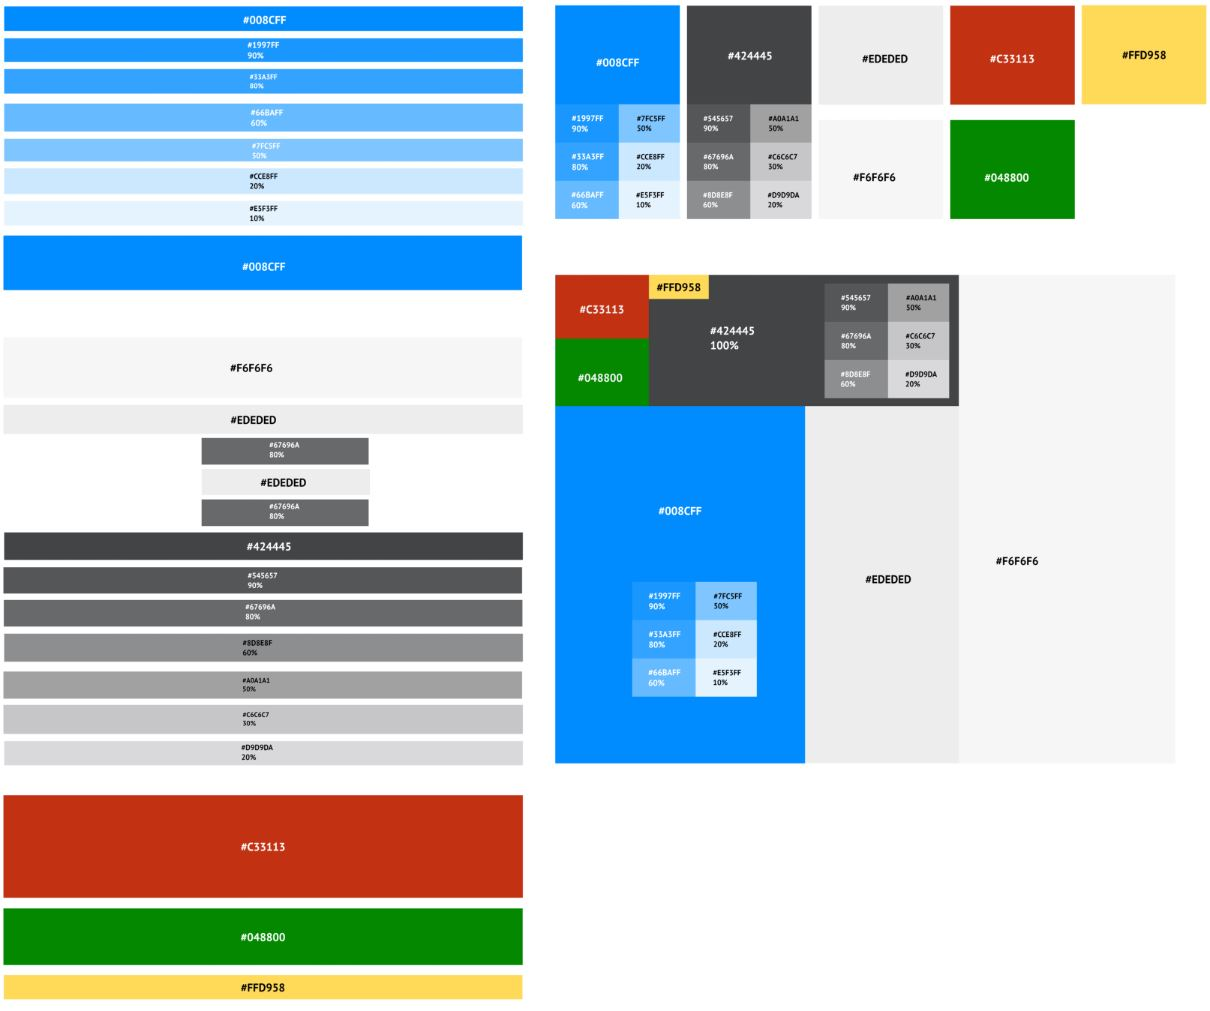
\includegraphics[width=100mm]{figures/Design-utforming/Fargepalett.JPG}
    \caption{Den komplette fargepaletten til Millum.}
    \label{fig:farger}
\end{figure}

\section{\textbf{Skisser og prototyper}} \label{Skisser}
I dette avsnittet går vi mer i dybden på skissene og prototypene vi lagde og hvordan disse utviklet seg til den endelig løsningen. \textit{Å lage skisser bidrar til å foreslå, utforske og formidle idéer (Rojas 2019).}

\section{\textbf{Designets evolusjon}}
Ved å jobbe i sprintsykluser hadde vi muligheten til å se evolusjonen av designuttrykket vårt underveis i hele prosessen. Som nevnt i \textbf{\ref{Skisser}} lagde vi lavnivå-skisser som viste ønsket funksjonalitet, men ikke pikselperfekte detaljer. Grunnen til at vi laget lavnivå-skisser er at vi hadde et ønske om å inkludere oppdragsgiver i prosessen ved å kontinuerlig få tilbakemeldinger på design og oppførsel.

I tredje sprint hadde vi mye av funksjonaliteten på plass og bestemte oss for å jobbe med en del av tilbakemeldingene vi hadde fått på sprintpresentasjonene. I eksempelet (\textbf{\ref{fig:evolusjon_dashboard}}) ser man hvordan designuttrykket har endret seg på tre sprintsykluser. 

\begin{figure}[H] 
    \centering
    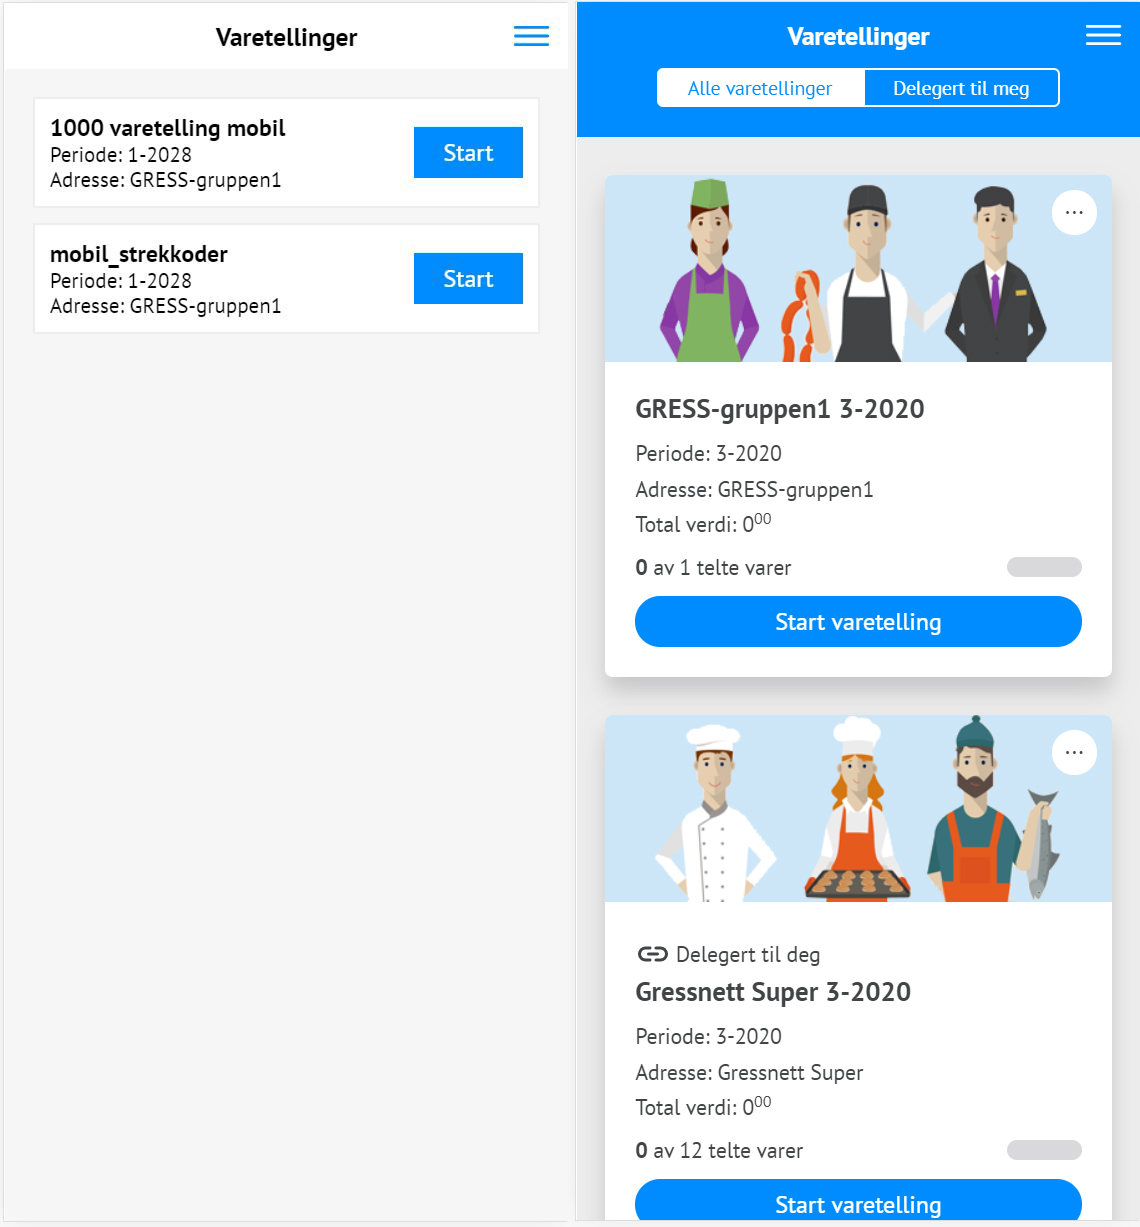
\includegraphics[width=100mm]{figures/Design-utforming/Evolusjon_dashboard.jpg}
    \caption{Dashboard i sprint 3 (t.v). Dashboard i sprint 6 (t.h).}
    \label{fig:evolusjon_dashboard}
\end{figure}

\section{\textbf{Design for flere flater}}
I samsvar med spørreundersøkelsen vi gjennomførte (\textbf{REF SPØRREUNDERSØKELSE}) så vi behovet for å utvikle løsningen for både mobil og nettbrett. Den åpenbare grunnen til å designe for flere flater er at vi støtter enhetene til flere i målgruppen, samt at vi kan utnytte plass bedre på større enheter. Eksempelvis ved å vise label og inputfelt ved siden av hverandre på nettbrett, men over/under på mobil som vist i figur \textbf{\ref{fig:tablet_vs_mobil}}. Vi skriver mer om universell utforming i neste avsnitt.

\begin{figure}[H] 
    \centering
    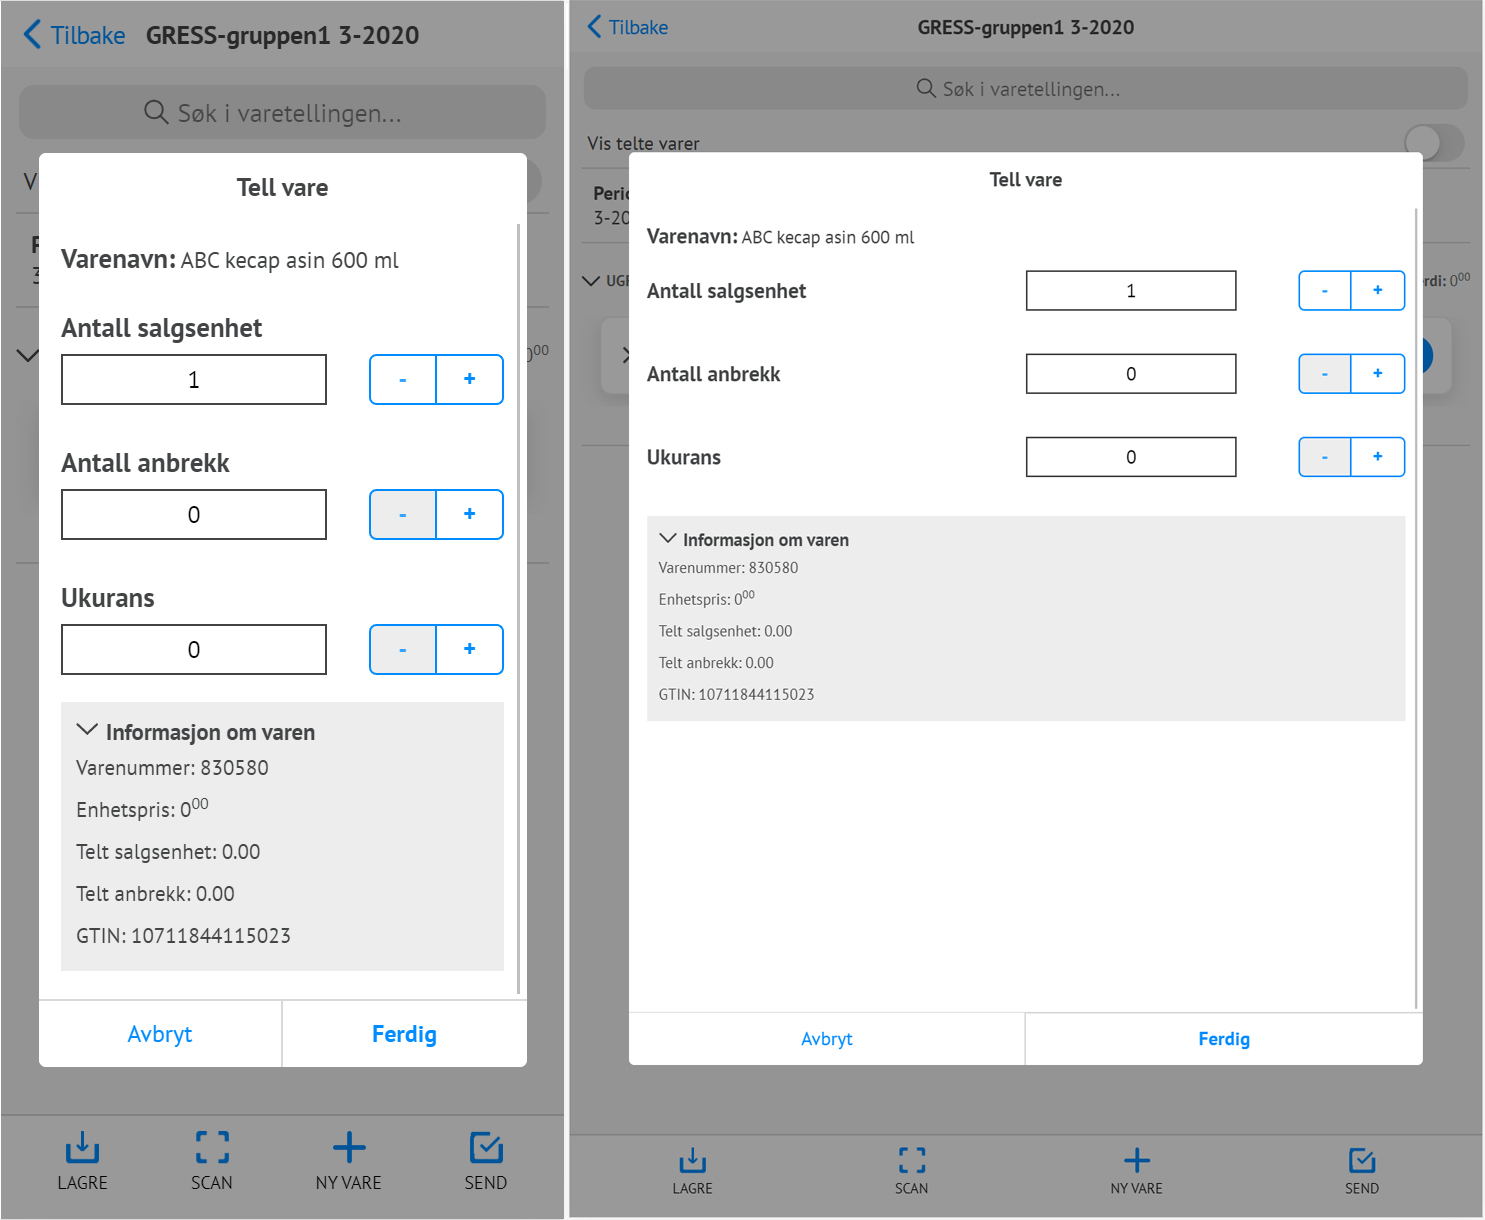
\includegraphics[width=100mm]{figures/Design-utforming/Tablet_vs_mobil.jpg}
    \caption{Mobilvisning av tellemodus (t.v). Nettbrettvisning av tellemodus (t.h).}
    \label{fig:tablet_vs_mobil}
\end{figure}

\section{\textbf{Universell utforming}} \label{Universell_utforming}
Universell utforming handler om å utforme omgivelsene slik at vi tar hensyn til variasjonen i funksjonsevne hos innbyggerne, inkludert personer med nedsatt funksjonsevne.\cite{digiuniversell} Hensikten er å kunne nå alle målgruppene gjennom en og samme løsning. Forskriften om universell utforming av IKT-løsninger stiller krav om at nettsider må oppfylle 35 av 61 suksesskriterier i “Retningslinjer for tilgjengelig webinnhold" \cite{digiwcag}. Mobilapplikasjonen vi har utviklet er omfattet da den må laste ned informasjon fra internett for å fungere.

Universell utforming er mer enn bare å tilrettelegge for mennesker med funksjonsnedsetting, men også eksempelvis mennesker med annet morsmål, lav domenekunnskap, vanskeligheter for å bruke mobiltelefon og så videre. Det har vært viktig for oss å ikke bare tenke på universell utforming, men aktivt inkludere det underveis i prosessen. Vi vet at mange av kundene til Millum har andre morsmål enn norsk og har derfor vært opptatt av å inkludere flere språk, selv om dette ikke var et formelt krav fra oppdragsgiver.

Det kan være vanskelig å følge alle retningslinjene, men det er lettere gjort når man inkluderer det i hele prosessen. Mange av våre designvalg har vært i tråd med artikler og forskning gjort av Nielsen Norman Group, som ansees for å være en av verdens fremste på forskningsbasert universell utforming og brukeropplevelse. Eksempelvis kan vi vise til det som kalles for \textit{input steppers}. Det vil si et inputfelt med tilhørende knapper for pluss og minus. 
\begin{figure}[H] 
    \centering
    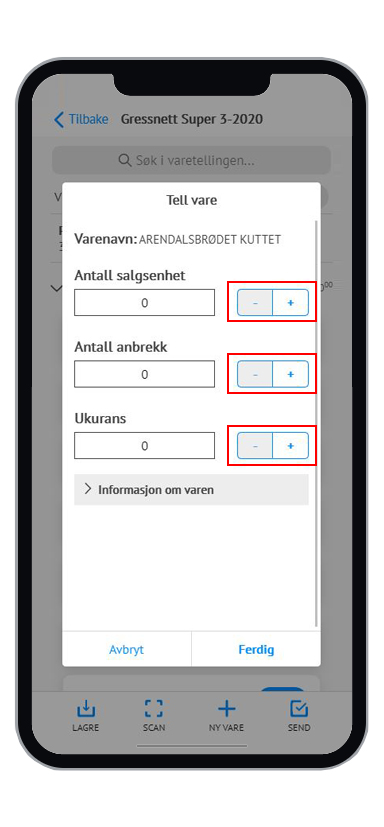
\includegraphics[width=75mm]{figures/Design-utforming/universell-utforming.jpg}
    \caption{Inputfelt (t.v). Input stepper markert i rød boks (t.h).}
    \label{fig:DesignInputStepper}
\end{figure}

En av de sentrale funksjonalitetene i løsningen er å kunne telle antallet man har av en vare. Vi var derfor helt avhengig av en god brukeropplevelse og har gjennom flere iterasjoner og bruk av forskning fra Nielsen Norman Group\cite{nngsteppers} kommet frem til en god måte å telle på. Ved å kunne taste inn store tall på eksempelvis vekt og volum, men samtidig kunne trykke en eller to ganger på en vare det ikke finnes mange av gir vi brukeren to valg og forenkler prosessen (\textbf{\ref{fig:DesignInputStepper}}). Universell utforming handler også om brukervennligheten, som vi kommer tilbake til i neste avsnitt om designprinsipper.

\section{\textbf{Designprinsipper}}
\subsection{\textbf{Bekreftelsesprinsippet}}
\textit{Bekreftelsesprinsippet er en teknikk brukt til kritiske handlinger, input eller kommandoer.}  (Lidwell 2003, s. 44)

Bekreftelse er en to-stegs operasjon som krever en handling fra brukeren i forkant av visning av dialogen. For å unngå at brukeren gjennomfører handlinger med katastrofale konsekvenser, som å gå ut av varetellingen uten å lagre bruker vi bekreftelsesdialoger for å hjelpe brukeren med å forstå konsekvensen av handlingen og gir de et valg om å likevel gjennomføre handlingen (som vist i \textbf{\ref{Bekreftelsesdialog}}).

\begin{figure}[H] 
    \centering
    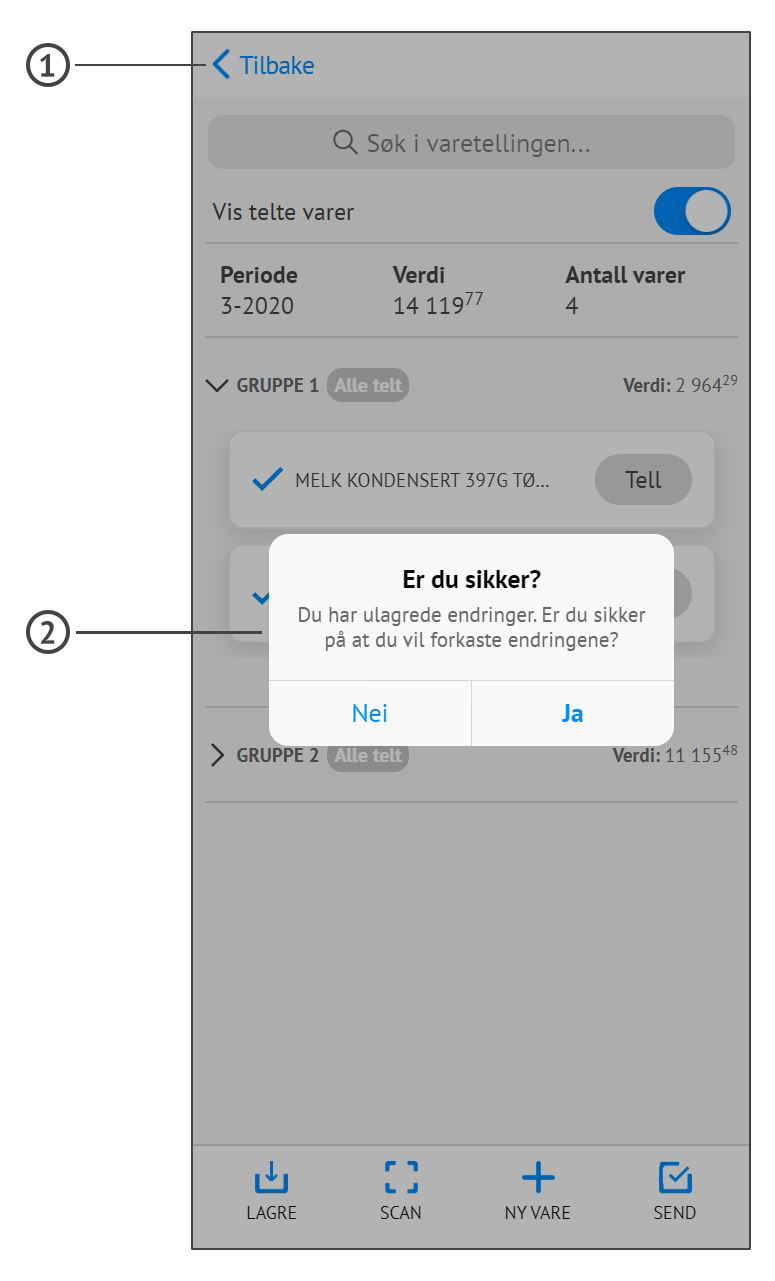
\includegraphics[width=75mm]{figures/Design-utforming/principle_confirmation.JPG}
    \caption{Bekreftelsesdialog (2) etter å ha trykket på tilbakeknapp (1) mens det foreligger ulagrede endringer}
    \label{Bekreftelsesdialog}
\end{figure}

\subsection{\textbf{Konsekvent design}}
William Lidwell skriver at brukervennligheten til et system forbedres når lignende deler uttrykkes på like måter. (Lidwell 2003, s. 46)

Ved å være konsekvent i design, tilbakemeldinger til brukeren, fargevalg, font o.l. Her økes ikke bare brukervennligheten i mobilapplikasjonen, men bygger også på helheten i produktporteføljen ettersom brukeren allerede kjenner til grensesnittet i handelsportalen Millum Procurement som vist i (\textbf{\ref{Konsekventdesign}}). 

\begin{figure}[H] 
    \centering
    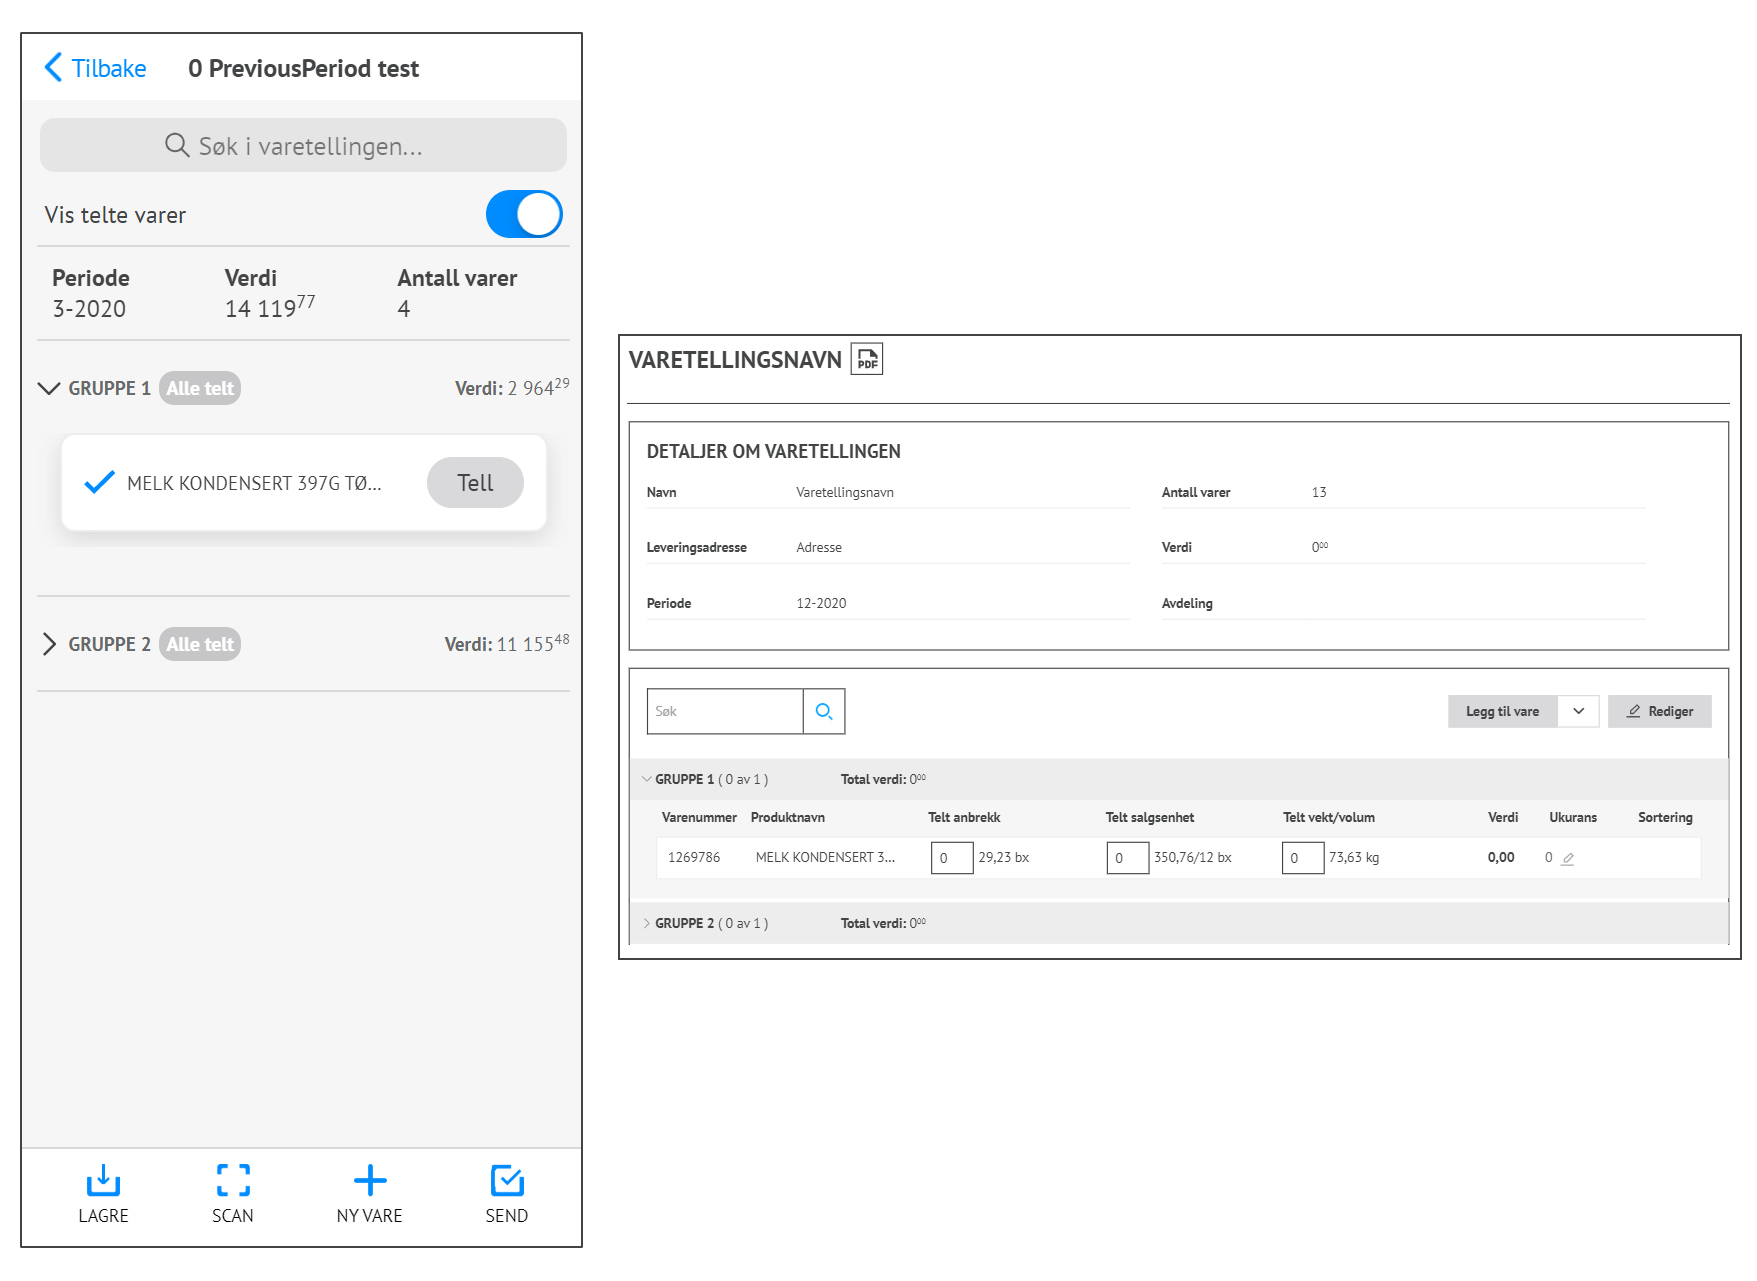
\includegraphics[width=150mm]{figures/Design-utforming/principle_consistency.jpg}
    \caption{Designuttrykk i mobilapplikasjonen (t.v) mot designuttrykket i webløsningen (t.h)}
    \label{Konsekventdesign}
\end{figure}

%%Avsnitt om flyt i applikasjonen med tanke på at vi konsekvent har valgt "3 sideer" slik at bruker kan effektivt navigere seg raskt igjennom arbeidet med å gjennomføre en varetelling
\subsection{\textbf{Proximity}}
\textit{Elements that are close together are perceived to be more related than elements that are farthel- apart.}(Lidwell 2003, s. 160).

Dette er et viktig prinsipp, siden feilvalg kan føre til frustrasjon for brukeren. Å gruppere elementer som hører sammen gjør det lettere for brukeren å forstå sammenhengen. Dette fører også tilbake til forrige punkt om konsekvent design. Dette ser vi flere ganger gjennom applikasjonen, eksempelvis i tellemodusen hvor et inntastingsfelt har tilhørende pluss- og minusknapper, eller i bunnmenyen hvor knappene har tilhørende tekst.

\subsection{\textbf{Chunking}}
Chunking er et prinsipp hvor formålet er å øke hukommelsen til brukeren i løsningen. Ofte blir en bruker overveldet av all informasjon man har tilgjengelig og prinsippet sier derfor at man bør bryte opp informasjon i mindre deler og konkretisere innholdet. Man må være sikker på at innholdet man lager er nødvendig og enkelt nok til å forstå slik at brukeren ikke bare oppfatter budskapet, men husker formålet med innholdet. Eksempler på hvordan vi har benyttet oss av dette prinsippet i løsningen vår er så enkle grep som å lukke seksjoner med informasjon som ikke er helt nødvendig å presentere for brukeren til enhver tid, som vist i figur \textbf{\ref{Informasjon_lukket}}

\begin{figure}[H] 
    \centering
    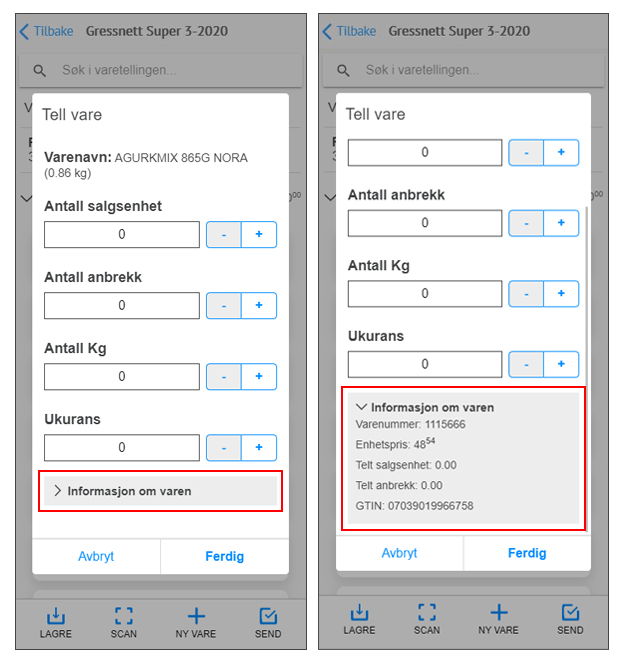
\includegraphics[width=100mm]{figures/Design-utforming/information_collapsed.jpg}
    \caption{Informasjon om varen lukket (t.v). Informasjon utvidet (t.h)}
    \label{Informasjon_lukket}
\end{figure}

\subsection{\textbf{Mapping}}
I denne konteksten betyr \textit{mapping} relasjonen mellom funksjonalitet og utseende. Trykker du på lysbryteren på veggen forventer du at lyset skrus av eller på, og ikke at du skrur på radioen. Dette gjelder også i design av produkter, og vi har vært bevisste på dette.

%Trykker du på en knapp forventer du kanskje en hvis form for funksjonalitet fra trykket i forhold til hvilket ikon eller tekst knappen er utsmykket med. For eksempel kan det tenkes at en knapp med et profil ikon åpner en profil side, med informasjon som: brukernavn, passord, gatenavn, innstillinger osv. Vi har brukt logisk Mapping ved å gi knapper ikoner og tekster (noe om logisk ikon bruk..). Et eksempel på dette... (sett in screen)

\section{\textbf{Brukervennlighet}}
 
 Brukervennlighet, eller \textit{Usability} på engelsk handler om hvor enkel løsningen er å forstå og å bruke. Man kan argumentere for at brukervennligheten er summen av de prinsippene vi har fulgt, ved å gjøre konkrete og gjennomtenkte designvalg gjennom hele prosjektet. I den moderne verden har brukervennlighet blitt viktigere enn noen gang, og om brukeren ikke forstår eller misliker innholdet så vil ofte brukeren slutte å bruke løsningen. Vi ønsker at brukeren skal oppleve verktøyet som intuitivt, og at arbeidsprosessen forbedres ved bruk av løsningen.
     
     %I den moderne verden har brukervennlighet blitt mer viktig enn noen gang. Om bruker ikke forstår eller misliker funksjonalitet til en applikasjon er det lett at bruker ikke vil fortsette å bruke applikasjonen. Vi leser ikke lenger manualer eller håndbøker ved bruk av applikasjoner.  I en studie medgir Google at hele 53\% av brukere forlater mobilapplikasjonen om siden tar over 3 sekunder å lastes inn(). I forhold til vår applikasjon er dette mindre relevant ettersom vår applikasjon er et arbeidsverktøy. Det viktigste er at arbeids prosessen utføres raskt og effektivt. Det er så klart også viktig at bruker liker arbeids verktøyet, spesielt ettersom vår applikasjon er et alternative, ikke en nødvendighet. %
     
     \textit{For intranets, usability is a matter of employee productivity. Time users waste being lost on your intranet or pondering difficult instructions is money you waste by paying them to be at work without getting work done.}(Jakob Nilsen, 3 Januar. 2012, NNGroup)
     
     
     
     
    
 
